


% svg debiliškai gaunas, sueis screeshot'as for the moment
% redaguoti galima čia https://demo.bpmn.io/s/start
% originalus failas: processes.bpmn

\begin{landscape}
\section{Procesų aprašymas}
Dokumente pateiktos diagramos sumodeliuotos naudojant BPMN 2.0 notaciją.
\thispagestyle{empty}
\begin{figure}[H]%[htpb!]
    \centering
    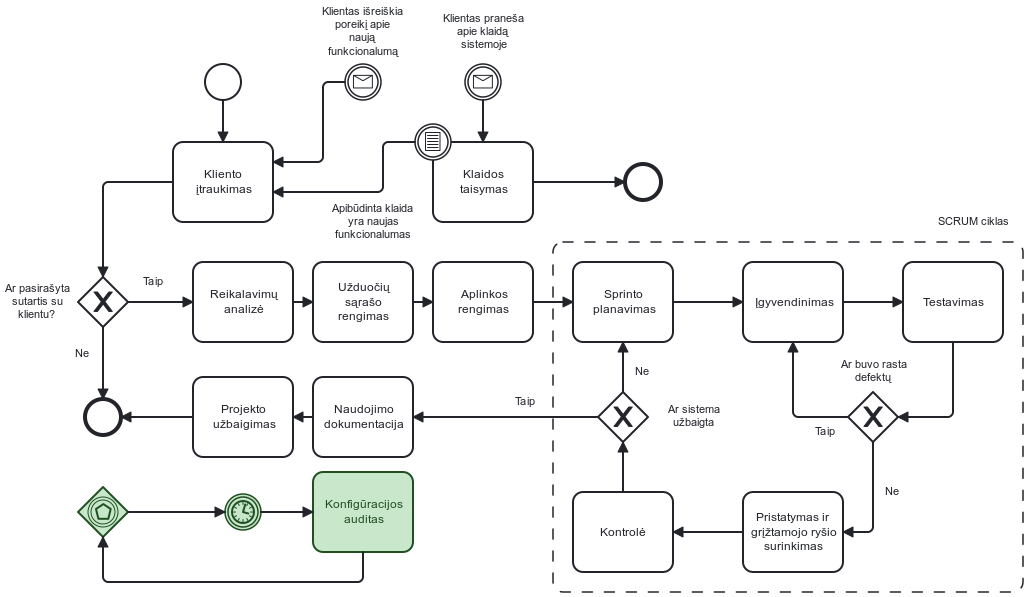
\includegraphics[width=0.85\linewidth]{./etc/diagrams/processes.png}
\end{figure}
\end{landscape}

\subsection{\process{EngageClient}} % ARNAS

\begin{figure}[H]%[htpb!]
    \centering
    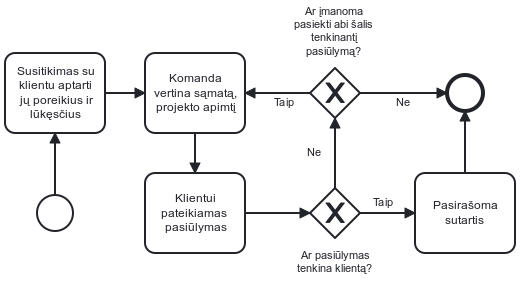
\includegraphics[width=0.75\linewidth]{./etc/diagrams/engage-client.png}
\end{figure}

\begin{processTable}{EngageClient}
    \tikslas{Siekiama įvertinti kliento poreikius, rasti kompromisą dėl projekto sąmatos bei apimties ir pasirašyti sutartį.}
    \inputs{

        \item \workProd{ClientNeeds} (šis darbo produktas yra išorinis)
        \item \hladd{\workProd{ClientReq} (šis darbo produktas yra išorinis)}
        \item \workProd{Experience}
        
    }
    \outputs{   
        \item \workProd{ResourceEstimates}
        
        \item \workProd{ProjectScope}
        
        \item \workProd{Contract}
        
        \item \workProd{Risks}
    }
    \veiklos{
         \item Projektų vadovas, architektas ir analitikas bendrauja su klientu, aiškinasi jo poreikius projektui (\workProdId{ClientNeeds}) \hladd{ir kliento reikalavimus projektui (KR)}. Ši veikla tęsiasi tol, kol įmonės atstovai surenka pakankamai informacijos paruošti klientui pasiūlymą.

        \item Projektų vadovas, architektas ir analitikas paruošia pradinę projekto viziją tam, kad būtų patvirtintas projekto įgyvendinamumas ir suderinta bendra projekto kryptis su SŠ. Jie taip pat atlieka pagrįstumo analizę, siekdami įvertinti, ar kliento poreikiai (KP) \hladd{ir kliento reikalavimai produktui (KR)} yra įgyvendinami.\label{activity:prepare-deal}

        \item Analitikas identifikuoja ir įvertina projekto rizikas, pagal jas sukuria rizikų valdymo planą (\workProdId{Risks}).

        \item Projektų vadovas, architektas ir analitikas  atsižvelgdami į projekto viziją, pagrįstumo analizę, departamento patirtį su kitais projektais (PAT) bei projekto apimtį (PA) nustato laiko, kainos ir žmogiškųjų išteklių sąmatą (IS). Laikas, kaina (nustatyti iš IS), projekto apimtis (PA), produkto perdavimo sąlygos ir adaptacinio laikotarpio terminas tuomet yra teisiškai įforminami sutartyje (KS).
        

        \item Klientui yra pateikiama sutartis (\workProdId{Contract}). Jei klientas yra patenkintas sutarties sąlygomis, pereinama prie sutarties pasirašymo \ref{activity:sign}. Klientas gali nesutikti su sutarties sąlygomis. Tokiu atveju vyksta derybos - klientas pateikia naujus poreikius (\workProdId{ClientNeeds}) ir \hladd{kliento reikalavimus projektui (KP), ir } dar kartą vykdoma veikla \ref{activity:prepare-deal}. Jei abi šalys nesugeba rasti kompromiso, procesas gali būti nutrauktas ir darbas su klientu netęsiamas.

        \item Pasirašoma sutartis su klientu (\workProdId{Contract}). \label{activity:sign}
    }
\end{processTable}

\newpage
\subsection{\process{RA}} % DOMANTAS

\begin{processTable}{RA}
    \tikslas{
    Išskirti funkcinius ir nefunkcinius reikalavimus, apibrėžti aukšto lygio architektūrą.
    }
    \inputs{
        \item \workProd{ProjectScope}
        \item \workProd{Contract}
    }
    \outputs{
        \item \workProd{FunReq}
        \item \workProd{NonFunReq}
        \item \workProd{HighLevelArch}
        \item \hladd{\workProd{ISD}}
    }
    \veiklos{
        \item \hladd{Analitikas renka informaciją iš kliento. Pagal tai modeliuoja verslo procesus ir identifikuoja konkrečius naudotojų poreikius. Jei kyla prieštaraujančių reikalavimų - sprendžia juos su atitinkamais SŠ.} 
        \item \hladd { Analitikas identifikuoja išorines sąsajas su kuriomis turės komunikuoti kuriama sistema. }
        \item\hladd{ Architektas analizuoja identifikuotas išorines sąsajas ir rašo išorinių sąsajų dokumentaciją (\prodWorkId{ISD}). }
        \item \hladd{Architektas ir analitikas apibrėžia funkcinius (\workProdId{FunReq}) ir nefunkcinius reikalavimus (\workProdId{NonFunReq}) iš identifikuotų naudotojų poreikių, modeliuojamų verslo procesų, projekto apimties (\workProdId{ProjectScope}) ir identifikuotų išorinių sąsajų.}
        \item Architektas sukuria aukšto lygio sistemos architektūrą (\workProdId{HighLevelArch}) atsižvelgdamas į apibrėžtus funkcinius (\workProdId{FunReq}) ir nefunkcinius reikalavimus (\workProdId{NonFunReq}).

        \item\hladd{Analitikas ir architektas atlieka analizę, aiškinasi ar iškelti funkciniai (FR) ir nefunkciniai (NFR) reikalavimai yra įgyvendinami ir patikrinami. Jei pasirodo, kad rinkinyje yra neįgyvendinamų arba nepatikrinamų reikalavimų, jie yra performuluojami. }

        \item \hladd{Analitikas daro analizę, bendrauja su SŠ, aiškinasi ar reikalavimų rinkinys yra pilnas ir būtinas. Jei pasirodo, kad rinkinys yra ne pilnas grįžtama prie pirmos veiklos.}
    }
\end{processTable}

\newpage
\subsection{\process{DraftBacklog}} % ARNAS

\begin{processTable}{DraftBacklog}
    \tikslas{Iš reikalavimų analizės rezultatų sudaryti projekto užduočių sąrašą.}
    
    \inputs{
        \item \workProd{FunReq}
        \item \workProd{NonFunReq}
        \item \workProd{HighLevelArch}
    }
    
    \outputs{
        \item \workProd{Backlog}
    }
    
    \veiklos{

        \item Architektas kartu su analitiku grupuoja susijusius funkcinius (\workProdId{FunReq}) ir nefunkcinius (\workProdId{NonFunReq}) reikalavimus bei skaido aukšto lygio architektūrą (\workProdId{HighLevelArch}) į panaudos atvejus arba bendro pobūdžio užduotis, kurios bendrai sudaro projekto užduočių sąrašą (\workProdId{Backlog}).

        \item Architektas kartu su analitiku detaliai aprašo užduotis, nurodydami kokie funkciniai (\workProdId{FunReq}) bei nefunkciniai (\workProdId{NonFunReq}) reikalavimai įeiną į konkrečios užduoties apimtį.
        \item Architektas kartu su analitiku nurodo užduočių priėmimo kriterijus, kuriais vadovaujantis galima  objektyviai įvertini ar užduotis yra įgyvendinta.
        \item Projektų vadovas, architektas ir analitikas prioritetizuoja projekto užduočių sąrašą (\workProdId{Backlog}) jį surūšiuodami.
        \item Kiekvienai užduočiai (PUS) priskiriamos priklausomybių žymos, nurodant, ar užduotis priklauso nuo kitų užduočių.
    }
\end{processTable}

\newpage
\subsection{\process{CICD}}

\begin{processTable}{CICD}
    \tikslas{Paruošti kodo repozitoriją. Automatizuoti kodo testavimo bei diegimo procesą.}

    \inputs{
        \item \workProd{HighLevelArch}
    }

    \outputs{
        \item \workProd{Environment}
        \item \workProd{Codebase}
        \item \hladd{\workProd{ConfigRepo}}
    }

    \veiklos{
        \item Architektas atsižvelgdamas į aukšto lygio architektūrą (\workProdId{HighLevelArch}) sukuria kodo repozitoriją, kurioje bus saugomas programinis kodas (\workProdId{Codebase}), trečių šalių bibliotekų ir diegimo konfigūracija. Pagal pasirinkto karkaso (pavyzdžiui: .NET, Spring Boot) šabloną  sukuria pirminį projekto programinį kodą.

        \item Architektas parengia saugyklą trečių šalių bibliotekoms saugoti.

        \item Architektas sukuria ir parengia testavimo aplinką (\workProdId{Environment}).

        \item \hladd{Architektas sukuria produkto konfigūracinių failų repozitoriją (KFR) ir parengia ją naudojimui.
        }

        \item \hladd{Architektas užtikrina, jog konfigūracinių failų repozitorijos (KFR) pagrindinė šaka būtų atnaujinama tik kai pakeitimą patvirtina projekto vadovas.
        }

        \item \hladd{Architektas su testuotoju atsižvelgia į kliento poreikius projektui - identifikuoja testavimo įrankius, kurie gali priklausyti nuo kliento operacinės aplinkos, būtinus testavimui ir dokumentuoja repozitorijos apraše.
        }

        \item \hladd{Architektas kartu su testuotoju apibrėžia operacinius scenarijus, aplinką, procedūras, įvestis ir išvestis, kurie tikrins realaus pasaulio sąlygas (našumą, saugumą ir pan.). Ši dokumentacija yra repozitorijos dalis.
        }

        \item Architektas ruošia trečiųjų šalių bibliotekų saugyklas ir konfigūruoja CI/CD - užtikrina, kad sukūrus naują programinio kodo versiją būtų paleidžiami automatiniai testai, jiems suveikus be klaidų, nauja produkto versija automatiškai sudiegiama į testavimo aplinką (\workProdId{Environment}).
    }
\end{processTable}

\newpage
\subsection{\process{ScrumCycle}}

\subsubsection{\process{Refinement}}

\begin{processTable}{Refinement}
    \tikslas{
        Sudaryti sprinto užduočių sąrašą.
    }
    \inputs{
        \item \workProd{Backlog}
        \item \workProd{SprintReviewDoc} (tik nuo antro sprinto)
        \item \workProd{StoryPointRange} (tik nuo antro sprinto)
    }
    \outputs{
        \item \workProd{SprintBacklog}
        \item \workProd{Backlog}
    }
    \veiklos{
        \item Projektų vadovas, kuris atsižvelgia į sprinto peržiūros ataskaitą (\workProdId{SprintReviewDoc}), nustato sprinto tikslus. Jei istoriniai praėjusių sprintų duomenys dar neegzistuoja, nes vykdomas pirmasis sprintas, atsižvelgiama į projektų užduočių sąrašo (\workProdId{Backlog}) pirminę prioritetizacija.
        \label{SP:1}

        \item Projektų vadovas, bendro komandos susitikimo metu, \ref{SP:1}  veikloje įvardintus tikslus paskelbia komandai. Į tai atsižvelgę komandos nariai gali atnaujinti projekto užduočių sąrašo (\workProdId{Backlog}) prioritetus. 
        
        \item Jei komandos nariai nusprendžia, kad tam tikra užduotis iš projekto užduočių sąrašo (\workProdId{Backlog})  turi būti išskaidoma į atomiškas užduotis, tai ir yra atliekama - skaidomai užduočiai sukuriamos vaikinės užduotys.
        
        \item Komanda kiekvienai neįvertintai užduočiai įvertina laiką ir pastangas, naudojant pasakojimo vienetus, įprastai sekančius Fibonači seką.  Tai atliekama remiantis kelių komandos narių darbine patirtimi ir bendru susitarimu. Tuomet projekto užduočių sąraše (\workProdId{Backlog}) esančios užduoties atributas -- pasakojimo vienetai -- keičiamas į nutartą skaičių.
        
        \item Projektų vadovas sukuria sprinto užduočių sarašą (\workProdId{SprintBacklog}) atrinkdamas aukščiausio prioriteto  užduotis iš projekto užduočių sąrašo (\workProdId{Backlog})  taip, kad jų bendra pasakojimo vienetų suma tilptų į pasakojimo vienetų intervalą (\workProdId{StoryPointRange}). Pirmojo sprinto metu, dar neturint pasakojimo vienetų intervalo, parenkama tiek užduočių, kiek komanda bendru nutarimu nusprendžia. Komanda peržiūri užduotis, kurios priklauso nuo kitų užduočių, užduočių sąraše (SUS) ir užtikrina jų tinkamą prioritetą užduočių sąraše (SUS). Sprinto užduočių sąrašas (\workProdId{SprintBacklog}) realizuojamas visai komandai ir SŠ matomomis „Kanban“ lentomis.
        
        \item Komandos nariai planuoja, kas atliks kurią sprinto užduotį. Nutarus, sprinto užduočių sąraše (\workProdId{SprintBacklog}) kiekvienos užduoties atributas -- atsakingas asmuo --  keičiamas į už užduoties įgyvendinimą atsakingo asmens vardą ir pavardę.
    }
\end{processTable}

\newpage
\subsubsection{\process{Development}}

\begin{processTable}{Development}
    \tikslas{
         Atlikti sprinto užduočių sąraše išvardytas užduotis.
    }
    \inputs{
        \item \workProd{SprintBacklog}
        \item \workProd{DefectReport}
        \item \workProd{Codebase}
        \item \workProd{TechDoc}
        \item \hladd{\workProd{ISD}}
    }
    \outputs{
        \item \workProd{SprintBacklog}
        \item \workProd{Codebase}
        \item \workProd{TechDoc}
        \item \hladd{\workProd{CodeReviewReport}}
    }
    \veiklos{
        \item Kiekvieną dieną komanda rengia trumpą Stand-Up susitikimą, kad aptartų progresą, nustatytų kliūtis ir sinchronizuotų veiklas tarp komandos narių. Šis susitikimas įprastai trunka ne ilgiau kaip 15 minučių ir susideda iš trijų pagrindinių punktų: kas buvo padaryta vakar, kas bus daroma šiandien, ir su kokiomis kliūtimis susiduriama.
        \item Kai programinės įrangos kūrėjai atlieka jiems priskirtą užduotį, užduoties statusas keičiamas IN PROGRESS. 
        \item Jei šis procesas vykdomas, kai užduotis buvo grąžinta į įgyvendinimą (\textit{ĮG}) po testavimo proceso (\textit{TE}), programinės įrangos kūrėjai atsižvelgia į klaidų aprašus (\workProdId{DefectReport}), kad ištaisytų klaidas. Kitu atveju veikla praleidžiama.
        \label{IG:2}

        \item Programinės įrangos kūrėjai pritaiko testų kūrimo metodą (TDD), prieš pradedant kurti funkcionalumą. TDD užtikrina, kad kiekviena funkcija būtų padengta modulių testais, siekiant išvengti klaidų ir garantuoti kodo kokybę. Laikoma, kad yra atnaujinamas programinis kodas (\workProdId{Codebase}).

        % \hladd{ Kiekvienas programinės įrangos kūrėjas rašo kodą, jei prireikia, naudoja išorinių sąsajų dokumentaciją (ISD), kad įgyvendintų priskirtą užduotį ir taip papildo programinį kodą (PK). }
        \item \hladd{ Kiekvienas programinės įrangos kūrėjas rašo kodą, jei prireikia, naudoja išorinių sąsajų dokumentaciją (\workProdId{ISD}), kad įgyvendintų priskirtą užduotį ir taip papildo programinį kodą (\workProdId{Codebase}).}

        \item Sudėtingas arba itin svarbias užduotis programinės įrangos kūrėjai dalinai atlieka porose. Darbo porose tikslas - dalintis žiniomis ir efektyvesnė kodo peržiūra.
        \label{IG:4}

        \item Jeigu rašant programinį kodą, programinės įrangos kūrėjui paaiškėja, kad šios užduoties jis negalės atlikti, nes pirma turi būti atlikta kita užduotis, programinės įrangos kūrėjas sprinto užduočių saraše (\workProdId{SprintBacklog}) pažymi užduotį, nuo kurios priklauso jo atliekama užduotis. Toliau šios užduoties įgyvendinimas nėra tęsiamas iki kol kitos užduoties statusas nepasikeičia į DONE.
        \label{IG:3}

        \item Programinės įrangos kūrėjas, atsakingas už užduotį, keičia užduoties statusą į \mbox{IN~REVIEW}. Auotomatiškai prasideda kodo integracija ir diegimas į testavimo aplinką (CI/CD). Jei integracija ar diegimas nesėkmingi (yra kodo konfliktų su pagrindine kodo šaka arba ne visi testai teigiami), užduoties statusas automatiškai grąžinamas į \mbox{IN~PROGRESS}, progrminės įrangos kūrėjas, atsakingas už užduotį ištaiso klaidas ir veikla kartojama tol, kol CI/CD įvyksta sėkmingai.
        \label{IG:5}

        % \hladd{ Užduotį, kuri yra IN REVIEW, kitas komandos narys peržiūri, komentuoja kodą. Tas pats komandos narys užpildo kodo peržiūros raportą (KPR).  Jeigu kitas komandos narys pareikalauja pakeitimų, pakeičia užduoties statusą į IN PROGRESS. Už užduotį atsakingas asmuo turi pakartoti 7-9 veiklas. }

        \item \hladd{Užduotį, kuri yra IN REVIEW, kitas komandos narys peržiūri, komentuoja kodą. Tas pats komandos narys užpildo kodo peržiūros raportą (KPR). Jeigu kitas komandos narys pareikalauja pakeitimų, pakeičia užduoties statusą į IN PROGRESS. Už užduotį atsakingas asmuo turi pakartoti \ref{IG:3} - \ref{IG:6} veiklas.}
        \label{IG:6}
        \item Kitam komandos nariui patvirtinus kodo kokybę, programinės įrangos kūrėjas pažymi, kad programinį kodą (\workProdId{Codebase}) galima testuoti - užduoties statusas keičiamas į TESTING, o atributas atsakingas asmuo  keičiamas į už užduoties testavimą atsakingo asmens vardą ir pavardę.  
        \label{IG:7}

        \item Vykdomas techninės dokumentacijos poreikio įvertinimas. Vertinama pagal šiuos kriterijus: \textbf{konfigūracija} -- ar užduoties rezultatas konfigūruojamas produkto konfigūraciniuose failuose, \textbf{išoriškumas} -- ar užduoties rezultatas pasiekiamas išoriniams vartotojams (pvz. API), \textbf{kritiškumas} -- užduoties rezultato poveikis bendram produkto funkcionalumui.

        \item Techninė dokumentacija užduočiai rašoma tik jei jos poreikio vertinimas teigiamas. Visą reikalingą techninę dokumentaciją (\workProdId{TechDoc}) parašo programinės įrangos kūrėjas.
        \label{IG:8}

        \item Laikas, praleistas atliekant \ref{IG:2}-\ref{IG:8} veiklas pažymimas sprinto užduočių sąrašo (\workProdId{SprintBacklog})  užduoties atribute  „kūrimo valandos“.
    }
\end{processTable}

\newpage
\subsubsection{\process{Testing}}

\begin{processTable}{Testing}
    \tikslas{
        Verifikuoti programinį kodą.
    }
    \inputs{
        \item \workProd{SprintBacklog}
        \item \workProd{DefectReport} (nuo antro sprinto)
        \item \workProd{Codebase}
        \item \workProd{TechDoc}
    }
    \outputs{
        \item \workProd{DefectReport}
        \item \workProd{SprintBacklog}
        \item \workProd{Codebase}
    }
    \veiklos{
        \item Kiekvienas testuotojas atlieka jam priskirtą užduotį kaip nurodyta sprinto užduočių saraše (\workProdId{SprintBacklog}). 
        \label{TE:1}
        \item Testuotojai testuoja užduoties programinį kodą (\workProdId{Codebase}) pagal užduoties aprašymą, kuriame nurodyti funkciniai ir nefunkciniai reikalavimai. Jie taip pat atsižvelgia į užduoties priėmimo kriterijus, kurie nurodyti viename iš užduoties atributų. Pagal patirtį arba pasitarę su kitais komandos nariais, testuotojai gali nuspręsti atlikti integracijos, našumo, saugumo, regresijos ir kitus testus. 
        \label{TE:2}
        \item Testuotojai rašo arba taiso klaidų aprašus (\workProdId{DefectReport}), kad jie atspindėtų programinio kodo kokybės būklę.
         \label{TE:3}

        \item Automatizuotus regresinius testus kuria ir rašo testuotojas, kuris yra atsakingas už testų kūrimo ir priežiūros procesą. Šie testai užtikrina, kad kodo pakeitimai nesukelia klaidų ir nepažeidžia esamo funkcionalumo. Laikoma, kad atnaujintas programinis kodas (\workProdId{Codebase}). 
         
        \item Jei šio proceso metu buvo rasta klaidų, užduotis grąžinama atgal į įgyvendinimo (\processId{Development}) procesą, kad programinės įrangos kūrėjai išspręstų klaidas. Testuotojas turi pakeisti užduoties būseną, kad sprinto užduočių sąraše (\workProdId{SprintBacklog}) būtų nurodyta, kad jos statusas IN PROGRESS, o atributas -- atsakingas asmuo -- keičiamas į už užduoties taisymą atsakingo asmens vardą ir pavardę. Jei šio proceso metu nebuvo rasta klaidų, užduoties statusas pakeičiamas į DONE. Tuomet automatiškai atnaujinamos visos nuo šios užduoties priklausomos užduotys – jų priklausomybės statusas pakeičiamas į nebeblokuojantį.
         \label{TE:4}

        \item Laikas, kuris buvo praleistas atliekant \ref{TE:2}-\ref{TE:4} veiklas pažymimas sprinto užduočių sąraše (\workProdId{SprintBacklog}) esančios užduoties atribute 
         „testavimo valandos“.
    }
\end{processTable}

\newpage
\subsubsection{\process{PartialDelivery}}

\begin{processTable}{PartialDelivery}
    \tikslas{
       Pristatyti suinteresuotoms šalims atliktą darbą ir surinkti grįžtamąjį ryšį.
    }

    \inputs{
        \item \workProd{Codebase}
        \item \workProd{Backlog}
        \item \workProd{Environment}
        \item \workProd{Product}
    }
    \outputs{
       \item \workProd{Feedback}
       \item \hladd{ \workProdId{StakeholderInterest} }
    }
    \veiklos{
        \item Programinės įrangos kūrėjas pristato naujasią produkto versiją (\workProdId{Product}), įdiegtą testavimo aplinkoje (\workProdId{Environment}), suinteresuotoms šalims. Tai gali vykti nuotoliniu būdu arba gyvo susitikimo metu, per kurį naudojami įvairūs informacijos radiatoriai pvz: skaidrės, projektoriai, rašomosios lentos ir t. t.

        \item \hladd{Projekto vadovas peržiūti suinteruotų šalių įsitraukimą. Jeigu kyla problemų, atlieka analizę ir nustato jų poveikį. Tai, projektų vadovas, surašo suinteresuotų šalių įsitraukimo ataskaitoje.}
        
        \item Komandos nariai išklauso SŠ atsiliepimus apie atliktą darbą. Aptaria visus trūkumus, galimus patobulinimus ir pakeitimus projekto užduočių saraše (\workProdId{Backlog}).
        
        \item Projekto vadovas surašo surinktus atisiliepimus į grįžtamojo ryšio registrą (\workProdId{Feedback}).
    }
\end{processTable}


\newpage
\subsection{\process{Requirements}}

\begin{processTable}{Requirements}
    
    \tikslas{ \hladd{Sekti funkcinių ir nefunkcinių reikalavimų pokyčius ir kokybę.}}

    \inputs{
    
        \item  \hladd{\workProd{FunReq}}
        \item  \hladd{\workProd{NonFunReq}}
        \item  \hladd{\workProd{Feedback}}
        \item  \hladd{\workProd{Risks}}
        
    }
    \outputs{
        \item  \hladd{\workProd{FunReq}}
        \item  \hladd{\workProd{NonFunReq}}
        \item  \hladd{\workProd{Feedback}}    
    }
    \veiklos{
        \item \hladd{Architektas ir analitikas pagal grįžtamojo darbo registrą (GRR) apmąsto, kaip gali keistis funkciniai reikalavimai (FR) ir nefunkciniai reikalavimai (NFR). }
        \item \hladd{Pagal rizikų valdymo planą (RVP) įvertina reikalavimų pokyčių rizikas.}
        \item \hladd{Klientai informuojami apie rizikas. Komandos nariai išklauso SŠ atsiliepimus apie rizikas ir  projekto vadovas surašo surinktus atisiliepimus į grįžtamojo ryšio registrą (GRR).}
        \item \hladd{Architektas ir analitikas Pakeičia funkcinius reikalavimai (FR) ir nefunkcinius reikalavimus (NFR). Jų pokyčiai ir pokyčių priežastys užregistruojami ir laikomi "Jira" platformoje.}
        \item  \hladd{Architektas ir analitikas sudaro atsekamumo matricą funkcinių reikalavimų (FR) ir nefunkcinių reikalavimų (NFR) pokyčių kokybei užtikrinti. Jei trūkumų yra, vėl vykdoma 3 ir 4 veikla.}
        \item \hladd{Projektų vadovas įvertina ar funkcinių reikalavimų (FR) ir nefunkcinių reikalavimų (NFR) pokyčiai gali pakeisti procesuose esančius darbo produktus ir veiklas, jei gali, jie yra pakeičiami.}
    
    }       

    
\end{processTable}

\newpage
\subsubsection{\process{Control}}

\begin{processTable}{Control}
    \tikslas{
        Įvertinti kaip sekėsi sprintas ir suderinti būsimų scrum ciklų patobulinimus.
    }
    \inputs{
        \item \workProd{DefectReport}
        \item \workProd{SprintBacklog}
        \item \workProd{ResourceEstimates}
        \item \workProd{StoryPointRange}
        \item \workProd{Feedback}
        \item \workProd{Backlog}
        \item \workProd{Risks}
    }
    \outputs{
        \item \workProd{SprintReviewDoc}
        \item \workProd{StoryPointRange}
        \item \hladd{ \workProd{Risks} }
    }
    \veiklos{
        \item Visi komandos nariai apmąsto sprinto eigą, aptaria, kas pavyko ir su kokiais sunkumais susidūrė. Komanda aptaria iškilusias užduočių priklausomybes (angl. blockers). Visi komandos nariai surašo savo atsiliepimus.

        \item \hladd{Architektas peržiūri techninėje dokumentacijoje (\textit{TD}) aprašytas vidines ir išorines produkto (\textit{PROD}) sąsajas ir, jei reikia, atnaujina projekto užduočių sąrašą (\textit{PUS}) pridėdamas į jį reikalingas sąsajų atnaujinimo veiklas.
        }
        
        \item Projekto vadovas peržiūri sprinto užduočių sąrašą (\workProdId{SprintBacklog}), palygina faktinį užduotims atlikti sugaištą laiką su kūrimo valandų įvertinimais ir parengia laiko valdymo ataskaitą atsižvelgdamas į likusį laiką iš pradinių sąmatų (\workProdId{ResourceEstimates}).

        \item \hladd{Projekto vadovas peržiūri sprinto užduočių sąrašą (SUS), į jį atsižvelgdamas, palygina faktinį užduotims skirtus žmogiškuosius išteklius su pradinėmis sąmatomis (IS), pagal tai paskaičiuoja kainos ir įdėtų pastangų ataskaitą.}

        \item \hladd{Analitikas analizuoja naują informaciją iš komandos narių atsiliepimų ir grįžtamojo ryšio registro, įvertina ar nepasikeitė esamos ir/ar neatsirado naujos projekto rizikos, pagal tai analizuoja rizikas ir atnaujina rizikų valdymo planą (\workProdId{Feedback}).} Projekto vadovas vykdo stebėseną ir esant reikalui švelnina rizikas arba vykdo žalos kontrolę pagal rizikų valdymo planą (\workProdId{Feedback})\hladd{, ir suinteresuotų šalių įsitraukimo ataskaitą (SŠĮA), papildomai informuodamas atitinkamas SŠ.}.

        % \item Projekto vadovas vykdo stebėseną ir esant reikalui švelnina rizikas arba vykdo žalos kontrolę pagal rizikų valdymo planą (RVP).

        \item Remiantis grįžtamojo ryšio registru (\workProdId{Feedback})\hladd{, kainos ir įdėtų pastangų ataskaita}  ir laiko valdymo ataskaita projekto vadovas atlieka projekto užduočių sąrašo (\workProdId{Backlog}) atnaujinimą, prireikus, užduočių prioritetų keitimą, pasakojimo vienetų intervalo (\workProdId{StoryPointRange}) patikslinimą. Šie pakeitimai fiksuojami sprinto peržiūros ataskaitoje (\workProdId{SprintReviewDoc}).
        
        \item \hladd{
            Remiantis komandos atsiliepimais, komanda ir projektų vadovas nustato komandos procesų pakeitimus, kurie įsigalioja nuo kito sprinto. Pakeitimai gali įtraukti naujas verifikacijos procedūras darbo produktams, jų priėmimo kriterijų naujinimus, kriterijų vertinimo slenkstines ribas.
        }

        \item Jei projekto užduočių sąraše (\workProdId{Backlog}) visų užduočių statusas yra DONE, pereinama prie naudojimo dokumentacijos (\processId{CreateManual}), o SCRUM ciklai šiam projektui nebetęsiami.
    }
\end{processTable}

\newpage
\subsection{\process{CreateManual}}

\begin{processTable}{CreateManual}
    \tikslas{Paruošti produkto naudojimo instrukciją, suprantamą naudotojams.}
    \inputs{
        \item \workProd{Backlog}
        \item \workProd{Product}
    }
    \outputs{
            \item \workProd{Manual}
    }
    \veiklos{
        \item Iš užduočių sąrašo (\workProdId{Backlog}) išrenkami panaudos atvejai. 
        \item Detaliai aprašomi visi žingsniai kiekvienam panaudos atvejui įgyvendinti naudojant produkto (\workProdId{Product}) iliustracijas. \label{CreateManual/1}
        \item Detaliai aprašomos visos produkto (\workProdId{Product}) funkcijos (t.\,y. kaip jomis pasinaudoti). \label{CreateManual/2}
        \item Iš \ref{CreateManual/1} ir \ref{CreateManual/2} veiklų rezultatų sudaromas struktūrizuotas, vientisas dokumentas - \prodWork{Manual}
        \item Atliekama produkto naudojimo instrukcijos (\workProdId{Manual}) validacija - paruoštas dokumentas peržiūrimas kolegų iš kitų padalinių, įsitikinama, jog instrukcija suprantama pirmą kartą produktą (\workProdId{Product}) naudojantiems žmonėms. \label{CreateManual/3}
        \item Kol netenkinamas \ref{CreateManual/3} punktas, atliekami naudojimo instrukcijos pakeitimai.
        }
\end{processTable}

\begin{figure}[!h]
    \centering
    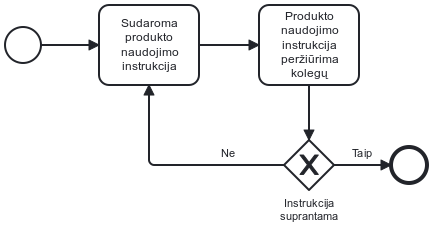
\includegraphics[width=0.75\linewidth]{./etc/diagrams/Manual.png}
\end{figure}
% --------------------------------------------------------------------
\newpage
\subsection{\process{CloseProject}}
\begin{processTable}{CloseProject}
    \tikslas{Užbaigti projektą, perduoti paruoštą naudojimui produktą klientams.}
    \inputs{
        \item \workProd{Product}
    	\item \workProd{Contract}
    	\item \workProd{Backlog}
    	\item \workProd{TechDoc}
    	\item \workProd{Manual}
        \item \hladd{\workProd{CodeReviewReport}}
    }
    \outputs{
        \item \workProd{Warranty}
        \item \workProd{Experience}
    }
    \veiklos{
        \item Atliekami sutartyje (\workProdId{Contract}) numatyti produkto (\workProdId{Product}) perdavimo klientui darbai.
        \item Klientui perduodama \prodWork{Manual}.
        \item Klientui perduodama \prodWork{TechDoc}.
        \item Sudaroma ir pasirašoma \prodWork{Warranty}, kurioje numatomas garantinio aptarnavimo laikotarpis.
        \item \hladd{ Analitikas atlieka kodo peržiūros raportų \prodWork{CodeReviewReport} analizę, identifikuoja pasikartojančias problemas ir bendro susitikimo metu jas adresuoja su kitais komandos nariais, taip prisidedama prie departamento patirties \prodWork{Experience} ugdymo. }
    	\item Atliekama vidinė komunikacija apie užbaigtą projektą. Projekto vadovas dalinasi projekto eiga, priimtais kritiniais sprendimais ir rezultatais. Taip kaupiama \prodWork{Experience}. 
    	\item Kol nesibaigia sutartyje (\workProdId{Contract}) numatytas adaptacinis laikotarpis, klientams teikiama techninė pagalba.
    }
\end{processTable}
\begin{figure}[!h]
    \centering
    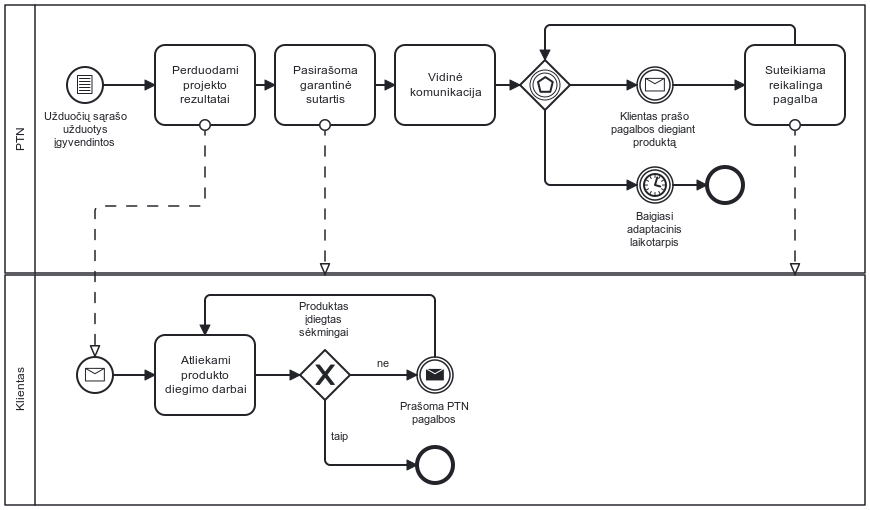
\includegraphics[width=0.8\linewidth]{./etc/diagrams/projectClosure.png}
\end{figure}

\newpage
\subsection{\process{ConfigAudit}}
\begin{processTable}{ConfigAudit}
    \tikslas{\hladd{Užtikrinti projekto konfigūracijos vientisumą.}}
    \inputs{
        \item \hladd {\workProd{ConfigRepo}}
        \item \hladd {\workProd{TechDoc}}
        \item \hladd {\workProd{Backlog}}
    }
    \outputs{
        \item \hladd{\workProd{Backlog}}
    }
    \veiklos{
        \item \hladd{
            Palyginama konfigūracijos repozitorijoje (KFR) esanti bazinė konfigūracija su techninėje dokumentacijoje (TD) aprašyta konfigūracija.
        }
        \item \hladd{
            Patikrinama, ar visi konfigūracijos nustatymai turi tinkamus identifikatorius ir yra minimi techninėje dokumentacijoje (TD).
        }
        \item \hladd{
            Patikrinama konfigūracijos repozitorijos (KFR) pakeitimų istorija ir užtikrinama, jog visi pakeitimai dokumentuoti ir susieti su projekto užduotimis, esančiomis projekto užduočių sąraše (PUS).
        }
        \item \hladd{
            Jei rasta neatitikimų, jie užregistruojami kaip atskiros užduotys projekto užduočių sąraše (PUS).
        }
    }
\end{processTable}

\newpage

%----------------------------------------


\subsection{\process{BugFix}}
\begin{processTable}{BugFix}
    \tikslas{Ištaisyti ne dėl kliento kaltės kilusias produkto klaidas.}
    \inputs{
        \item \workProd{Product}
    	\item \workProd{TechDoc}
    	\item \workProd{Contract}
    	\item \workProd{Warranty}
    	\item \workProd{Ticket} (išorinis darbo produktas)
    	\item \workProd{Manual}
     }
    \outputs{
        \item \workProd{Ticket}
        \item \workProd{Product}
    }
    \veiklos{
        \item Atliekama pirminė užregistruotos klaidos (\workProdId{Ticket}) analizė.
	   \item Jei užregistruota klaida (\workProdId{Ticket}):
            \begin{enumerate}[label=\alph*)] 
        		\item kyla dėl produkto (\workProdId{Product}) naudojimo nesilaikant produkto naudojimo instrukcijos (\workProdId{Manual})
        		\item kyla eksploatuojant produktą (\workProdId{Product}) netinkamomis, t.\,y. neatitinkančiomis techninės dokumentacijos (\workProdId{TechDoc}), sąlygomis
        		\item yra ne klaida, o neegzistuojančio ir sutartyje (\workProdId{Contract}) nenumatyto funkcionalumo įgyvendinimo prašymas
        		\item neatitinka garantino aptarnavimo sutartyje (\workProdId{Warranty}) numatytų sąlygų
        		\item yra užregistruota po garantino aptarnavimo sutartyje (\workProdId{Warranty}) numatyto garantinio laikotarpio
            \end{enumerate}
            tuomet užregistruota klaida (\workProdId{Ticket}) nėra taisoma ir šis procesas (\processId{BugFix}) yra užbaigiamas nevykdant tolesnių veiklų.
    	\item Atliekama klaidos kilimo priežasties analizė (root cause analysis).
    	\item Kuo įmanoma greičiau ištaisoma klaida ir sukuriama nauja produkto (\workProdId{Product}) versija.
    	\item Nauja produkto (\workProdId{Product}) versija perduodama klientams.
    	\item Užregistruota klaida (\workProdId{Ticket}) „Jira“ platformoje papildoma su klaidą ištaisančia prdoukto (\workProdId{Product}) versija bei klaidos kilimo priežastimi.    
    }
\end{processTable}
\newpage

%----------------------------------------

% \begin{processTable}{PrimaryKey}
%     \tikslas{}
%     \inputs{
%        \item \workProd{Kazkas}
%     }
%     \outputs{
%        \item \workProd{Kazkas}
%     }
%     \veiklos{
%         \item Kazkokia veikla
%     }
% \end{processTable}


%----------------------------------------